\documentclass[fleqn, 15pt, lineno]{olplainarticle}
% Use option lineno for line numbers 

\usepackage[T1]{fontenc}
\usepackage{mathptmx,placeins,lineno,setspace,fancyhdr,amsmath,textcomp,multirow,array,booktabs,gensymb,geometry,graphicx,arydshln,amssymb,siunitx}
\usepackage{colortbl}
\nolinenumbers

\title{Miscanthus hybridisation through field flowering synchronisation: methods to manipulate \textit{\textit{M. sinensis}} flowering to maximise seed yield}

\lhead{Awty-Carroll et al.,} 

\author[a*]{Danny Awty-Carroll}
\author[ab]{Antonella Iurato}
\author[c]{Danilo Scordia}
\author[a]{Giovanni Scalici}
\author[ad]{John Clifton-Brown}
\author[e]{Reza Shafiei}
\affil[a]{Institute of Biological, Environmental and Rural Sciences, Gogerddan, Aberystwyth University, Ceredigion, UK}
\affil[b]{Terravesta, Lincoln, UK}
\affil[c]{Catania university}
\affil[d]{Justus Liebig University Giessen, Germany}
\affil[e]{University of Dundee at JHI, Dundee, UK}
\affil[*]{Corresponding author: ani9@aber.ac.uk}

\keywords{Miscanthus, \textit{M. sinensis}, Flowering synchronisation, flowering delay}
%# Michal Mos?

\begin{abstract}
\linenumbers
\doublespacing
\textit{Miscanthus} is a high yielding second generation biomass crop, traditionally planted by clonal rhizome, seed based \textit{Miscanthus} is accelerating to meet the needs of the bio-economy.
Most of this seeded \textit{Miscanthus} is a hybrid of \textit{M. sinensis} and \textit{M. sacchariflorus}, this requires interspecies flowering synchronisation, which if not optimal significantly impacts seed quantity.

Changing the flowering time of ether parent may be required as, investment is required to grow \textit{Miscanthus} in pollen isolation and the flowering time changes as the perennial grass matures.
In this study, three treatments where tested on \textit{M. sinensis} to delay the flowering, 
cutting back the plants, adding nitrogen, and droughting them. 
Hybridisation crossing fields have also been established yet fail to yield adequately.
Remediation of low seed set by optimising planting densities and ratio of seed parents to pollen parents and trying supplemental misting treatments.
The effect on flowering time, seed set and seed quality was analysed.

We conclude that, while only cutting had a significant effect on flowering time, its effect on seed quantity and quality make it not useful for  , other promising treatments had less effect on seed quantity and quality.

\end{abstract}


\begin{document}


\flushbottom
\maketitle
\thispagestyle{empty}


%%%%%%%%%%%%%%%%%%%%%%%%%%%%%%%%%%%%%%%%%%%%%%%%%%%%%%%%%%%%%%%%%%%%%%%%%%%%%%%%%%%%%%%%%%%%%%%%%%%%%%%%%
\doublespacing
\linenumbers
\section{Introduction}

\textit{Miscanthus} is a genus of perennial Asian grasses that have been utilised as a second generation biomass crops. 
This crop is is increasingly diversifying away from a single clone \textit{Miscanthus $\times$ giganteus}, in favour of seed based hybrids \citep{Clifton-Brown2019_progress}. 
Seed based \textit{Miscanthus} is much more saleable than clonal \textit{Miscanthus $\times$ giganteus}, however making the seeds at scale is still a novel problem. 
Efficient seed production relies on maximising seed parents while allowing pollen to easily reach all seed parents. 

The amount of seed required to make a climate impact in the UK alone would be 30,000 ha per year of additional biomass crop per year by 2035 \citep{Sixth_Carbon_Budget}. 
In order to achieve this number of \textit{Miscanthus} plants, 1.8 billion seeds would need to be produced annually. 
This would be when planting 20,000 plants per ha \citep{CliftonBrown2001,Rusinowski2019}, and sowing 3 seeds per plug plant when planting \citep{AwtyCarroll2020}. 
Seed production has been approximated to 2,000:1 \citep{Astley2017} which is a high but not maximum level of seed production, at this level 90 ha of seed production would be required. 
In maximising the seed per m$^2$ within a crossing block there is the ability to make production of commercially relevant seed quantities possible in smaller locations.

New commercial seeds based \textit{Miscanthus} is made from interspecies hybridisation this requires that \textit{M. sacchariflorus} and \textit{M. sinensis} to flower approximately at the same time.
Fortunately \textit{Miscanthus} is self incompatible \citep{HIRAYOSHI1955,Jiang2017} so a set of M. sacchariflorus and a set of M. sinensis clones together in a field will only produce interspecies seed.
This cross would make two interspecies hybrids made, of which only one would be is the selected hybrid. 

Much of \textit{Miscanthus} flowering initiation is a combination of day-length/photoperiod and temperature \citep{Jensen2013,Jensen2011a}, however there is also an influence of maturity that can have a large affect in the field.
Plants flowering at a similar time will produce some seeds, but being able to invoke optimal synchronisation produces more higher quality seeds.


> add Why sinensis x sacchariflorus?


%%%%%%%%%%%%%%%%%%%%%%%%%%%%%%%%%%%%%%%%%%%%%%%%%%%%%%%%%%%%%%%%%%%%%%%%%%%%%%%%%%%%%%%%%%%%%%%%%%
\FloatBarrier
\section{Materials and methods}
Methods such as varying planting density and increasing the ratio of seed parent to pollen parent to improve the total production in crossing plot (called a block), would allow more economic scaling of \textit{Miscanthus} by seed which is already 1,000 to 2,000 times scaling per ha, well over the 10-30 times scaling of rhizome \citep{Astley2017}.

Many crossing blocks have been setup and tested at a 37$^{\circ}$N latitude site (Sicily Italy), in collaboration with with Catania University.
Most irrigated \textit{Miscanthus} plants will flower at this latitude, however the problem for producing interspecies hybrids is getting the plants to flower at the same time.

All these trials required accurate flowering scores in order to assess the synchronisation and determine if a good seed set was possible.
Phenological flowering assessments were developed for this study based on practical experience, they do however, match the 40, 53, \& 60 in the Biologische Bundesantalt, Bundessortenamt and CHemische Industrie (BBCH) scale of \textit{Miscanthus $\times$ giganteus} (M$\times$g) morphological development stages \citep{Tejera2017}.
The custom protocol was extended in the second and third year to 12 stages to better account for the amount of the plant flowering and mach more of the BBCH scale (Table \ref{tab:FS}).

\begin{table}[ht]\tiny
\renewcommand{\arraystretch}{1.3}
\caption{A table of flowering scores used in 2017 \& 2018.
The subset of scores used in 2016 are highlighted in grey.}
\centering
\begin{tabular}{l  c}
\toprule
\textbf{Description} & \textbf{Flowering score}\\
\midrule
					Any flag leaf emergence 							&\textbf{1}\\
\rowcolor[gray]{.9} 10\% of plants/tillers have flag leafs 				&\textbf{1a}\\	
					$>$50\% of plants/tillers have flag leafs 			&\textbf{1b}\\	
\rowcolor[gray]{.9} Some plants in a plot have panicle $>$ 1cm			&\textbf{2}\\
					$>$ 50\% of plants in a plot have panicle $>$ 1cm	&\textbf{2a}\\
\rowcolor[gray]{.9} First Visible anthers on panicles					&\textbf{3}\\
					Stigma Visible										&\textbf{3a}\\
					Stamen Visible										&\textbf{3b}\\
					Swollen or colour change							&\textbf{3c}\\
					50\% of stems reached anthesis						&\textbf{4}\\
					$>$ 75\% of stems reached anthesis					&\textbf{4a}\\
					Flowering complete									&\textbf{5}\\
\toprule
\end{tabular}
\label{tab:FS}
\end{table}


Three trials in the southerly latitude of Catania (37$^{\circ}$24'32.436", 15$^{\circ}$3'36.72") were undertaken to determine planting configuration for optimum seed yield and test methods of improving the flowering synchronisation between \textit{M. sinensis} the seed parent and \textit{M. sacchariflorus} the pollen parent.
During each flowering season flowering stage was scored on the flowering scale in Table \ref{tab:FS} indicating progression from flag leaf to seed set.
When the seed was ripe the total number of panicles in each subsample was counted, and the seed collected.
Sub-samples of the seed from each trial were studied for size, density and germination.

Seed germination was conducted at 25$^{\circ}$C in constant light low (<15 PAR) for 12 days in both 2017 and 2018. 


\FloatBarrier
\subsection{Maximising seed yields}
\subsubsection{Changing quantity of seed parents}

\title{Ratio experiment}

A field trial to assess the affect of seed parent to pollen parent ratio was planted in 2016. 
This trial attempted to maximise seed production capacity through increase of the maternal seed parent.
This was done by adding extra lines of seed parents between double lines of pollen parents (Figure \ref{fig:RatioPlan}).
In the first year all the \textit{M. sacchariflorus} pollen parent were cut back in May to keep the heights aligned, in the second year, to measure the effect of this, only half of the pollen parent were cut in a crenelated style down the columns (Figure \ref{fig:RatioPlan}).

\begin{figure}
\centering
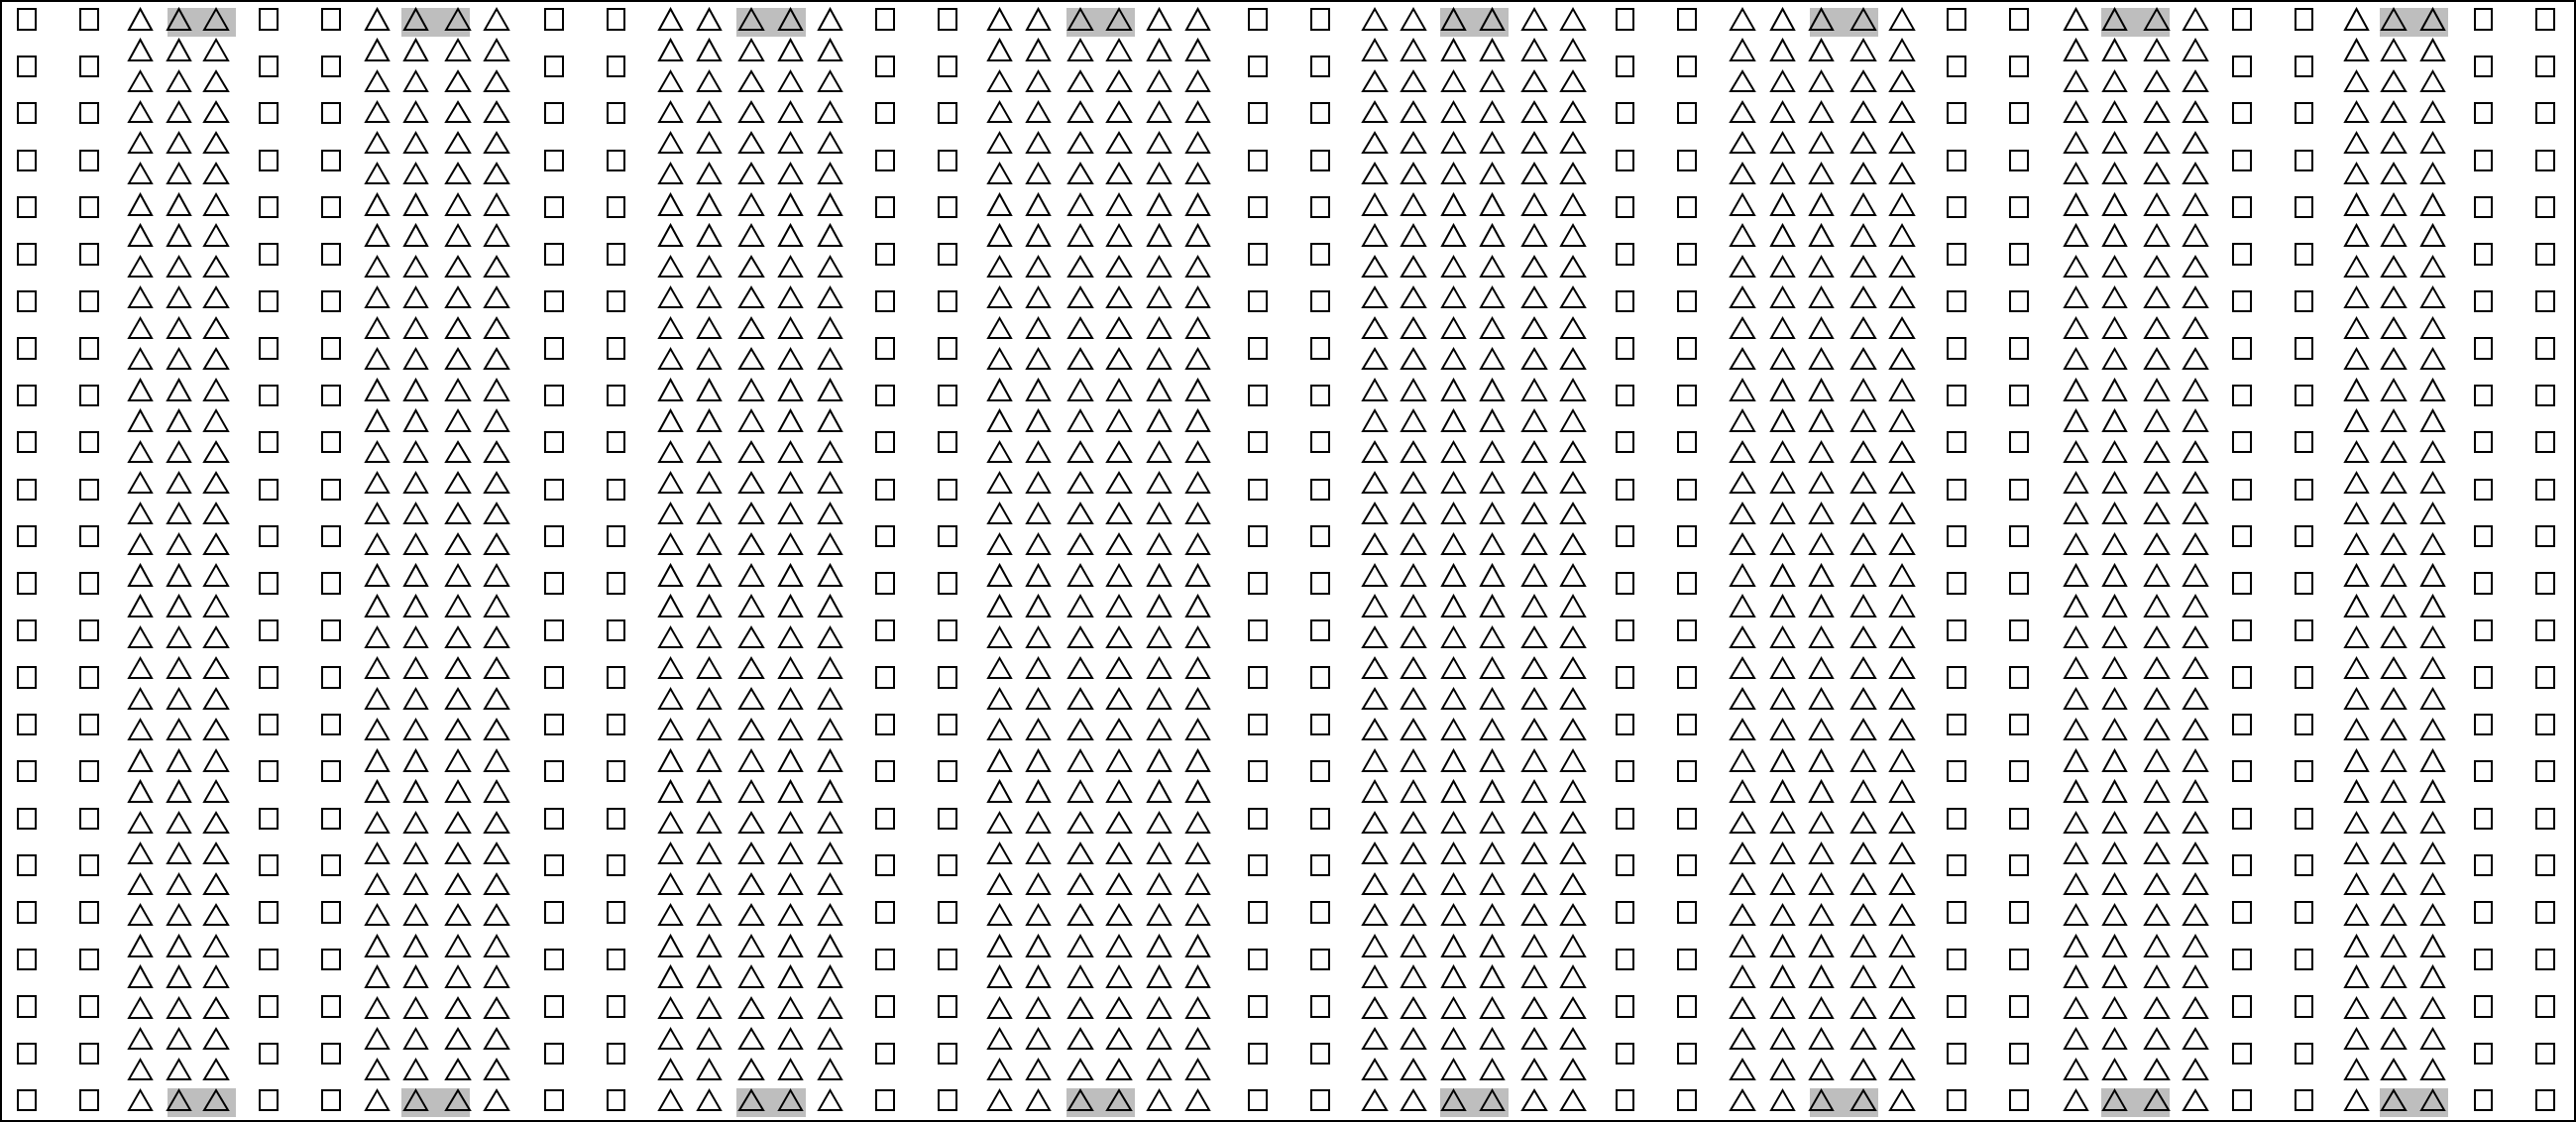
\includegraphics[width=1\textwidth]{Figs/CAT22Plan}
\caption{\label{fig:RatioPlan} A to scale plan of the ratio trial, the seed parent is shown as a $\bigtriangleup$ with the pollen parent as a $\Box$.
Due to the planting density when sub-samples were taken they were taken from the grey sections at the edge of the field.}
\end{figure}

This ratio trial was run for two years, flowering scores and seed weights were taken in both 2016 and 2017.
The data was averaged within each of the eight ratio sections was then used with two replicates for each ratio.

In the first year 10 plants were monitored from each side in each ratio (40 plants per ratio total) to assess the heights and the number of panicles.
In the second year the first linear meter of the rows highlighted in Figure 4 was collected as a subsample to allow a calculation of the amount of seed per m$^2$.
This change in methodology was due to the density, particularly as the planting density had resulted in lodging of the \textit{M. sinensis} during the second year, reducing the ease of access to the plot.
The data was analysed with R \citep{RCoreTeam2015}.


\FloatBarrier
\title{Density experiment}

If closer planted seed parents result in more seed in a smaller area this could allow more seed production of \textit{Miscanthus} interspecies hybrids.
Through moving the plants closer together there should be more panicles and therefore more seed per m$^2$ of crossing block.
Though this may increase stress and resource competition among the plants this should still produce a net increase in panicle numbers.
Also by using a denser crossing block the pollination may be expedited with more chance of the pollen getting to a seed parent.

\begin{figure}
\centering
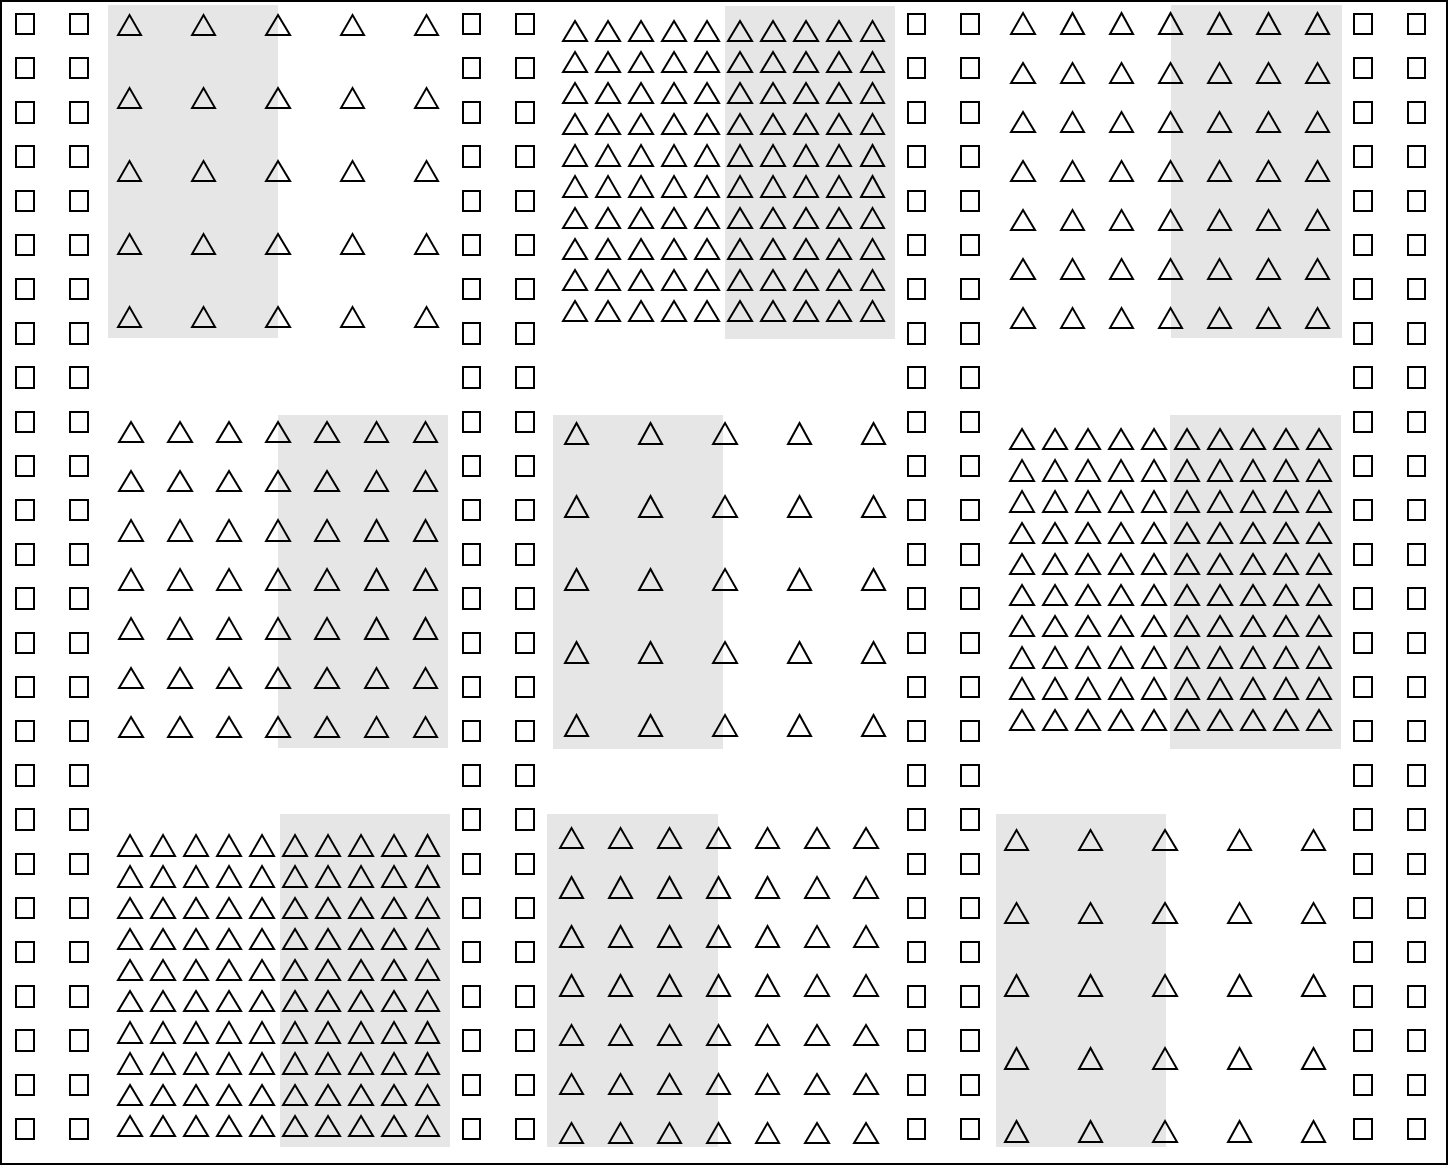
\includegraphics[width=0.82\textwidth]{Figs/CAT26Plan}
\caption{\label{fig:DensityPlan} A to scale plan of the density trial, the seed parent is shown as a $\bigtriangleup$ with the pollen parent as a $\Box$.
The densities used were 1, 2, and 4 seed parents per m$^2$, randomised three times into nine 25 m$^2$ blocks.
In 2018 only there was a pollen parent cutting treatment, shown as shading over a random half of each block within the crossing block.}
\end{figure}

To test this a trial was planted in 2016, using three densities of the \textit{M. sinensis} seed parent planting at 1, 2, and 4 plants per m$^2$.
These were planted in four randomised replicate blocks of 25 m$^2$ each with two row borders of the pollen parent at the edge of each block (Figure \ref{fig:DensityPlan}).

In all three years the \textit{M. sacchariflorus} pollen parent was cut back (late-May), to align heights.
Throughout the three years of the planting density trial panicles were collected to calculate the panicle number and seed amount per m$^2$. In the 3$^{rd}$ year due to the lodging the number of tall plants per plot needed to be reduced.
This was done using a cutting treatment to change the flowering time (`Cutting sinensis to synchronise flowering').



\FloatBarrier
\subsubsection{Misting to improve pollination}
A two factor trial (Figure \ref{fig:twoFactorPlan}) with a three block design was planted in 2015 and used to test two treatments per year for three years following an establishment year.
The plants were spaced at 0.66 plants per m$^2$, with rows of the \textit{M. sinensis} seed parents and \textit{M. sacchariflorus} pollen parents equally spaced (Figure \ref{fig:twoFactorPlan}).
In the second and third years the three cross sections of the field had three misting treatments; control, ground level and canopy level (3 m).
Six cuttings of the \textit{M. sacchariflorus} pollen parent were performed in the other direction in the second year (Figure \ref{fig:twoFactorPlan}).
In the third year a drought was also applied to the \textit{M. sacchariflorus} side of the hybrid.
This was only due to the practical construction of the trial (with alternating rows) as the \textit{M. sacchariflorus} did not need delaying to synchronise.

\begin{figure}
\centering
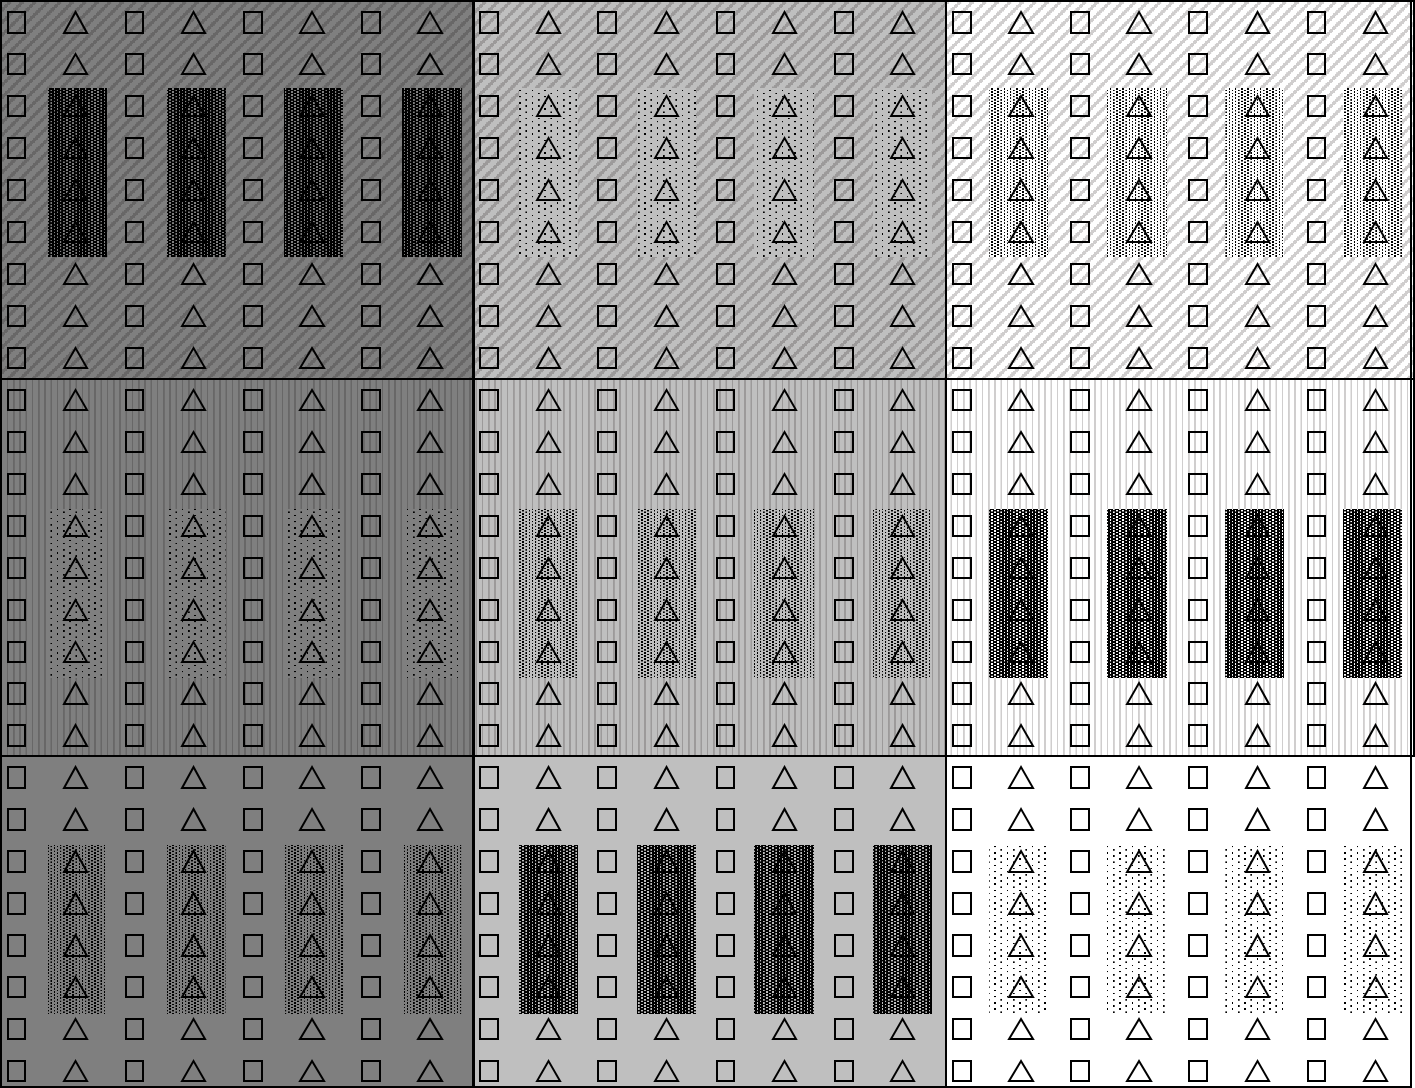
\includegraphics[width=1.1\textwidth]{Figs/CAT20Plan}
\caption{\label{fig:twoFactorPlan} A to scale plan of the two factor trial over the four years from planting.
The seed parent is shown as a $\bigtriangleup$ with the pollen parent as a $\Box$.
Nitrogen treatments are shown as dotted boxes over four plants in the centre of each treatment (used in 2017 \& 2018), these are from lightest to darkest: Control, 65 kg ha$^{-1}$, and 130 kg ha$^{-1}$.
The three horizontal sections represent misting used in 2016 \& 2017 (3rd \& 4th years); 3 m morning mist (diagonal shading), ground level morning mist (horizontal shading), and control (no shading).
The three vertical sections represent droughting used in 2018; these are shaded from darkest to lightest for drought levels induced by watering to replace only a percentage of evapotranspiration 25\%, 50\% and control (100\%).
This shows the nine sections the trial was divided into and the sub-sampling zones coloured where the second treatment was applied.
The plan alternates rows of \textit{M. sacchariflorus} and \textit{M. sinensis} at 1.5 m spacing.}
\end{figure}


This misting was applied in the second and third years of the two factor trial.
We hypothesise the morning misting will increase pollination and therefore seed set \citep{Clifton-Brown2018_pcb}.
To check the effect on the micro-climate of the misting, in the second year TinyTags (Gemini Data Loggers Ltd, Chichester, UK) collected relative humidity data averaged for each hour of the day from the 17/10/17 to 07/11/17.

The seed per m$^2$ gives the average amount of seed from a m$^2$ of \textit{M. sinensis} parents (seed parent).
Plant height was not measured in the 4th year as there was a lot of random variation in the other years.
The amount of seed per m$^2$ was calculated in the 4th year form an 80 panicle sub-sample.
n = 3


\FloatBarrier
\subsection{Delaying flowering to improve synchronisation}
As PCH-14 has poor flowering synchronisation between the \textit{M. sinensis} seed parent and the \textit{M. sacchariflorus} pollen parent and was a leading prospect for a commercial \textit{Miscanthus} hybrid in 2015, it was the therefor a logical choice to test for methods of altering flowering time in field conditions.
The information learned from from PCH-14  can also be applied to other crosses as interspecies hybridisation is the current route to market for new \textit{Miscanthus} varieties \citep{Clifton-Brown2019_progress}, \citep{Clifton-Brown2016_progress}.

Interspecies hybrid seed also provides the challenge of synchronising the flowering in two species growing in the same location \citep{Xue2015}.
Flowering synchronisation is predictable from year to year as often \textit{Miscanthus} flowering order is consistent across genotypes in multiple years \citep{Jensen2011}, apart from the first year.
If good flowering synchronisation is not possible in the location it may need one side to be modified, this could be done by using fertilisation, cutting or drought to induce flowering early, or trying various methods to slow the plant down.



\FloatBarrier
\subsubsection{Cutting sinensis to synchronise flowering}
Cutting can be done both to increase pollination by levelling the height difference between the \textit{M. sacchariflorus} and \textit{M. sinensis} and separately to change flowering time in the \textit{M. sinensis} seed parent.
This was dependent on the parent.

The density trial (Figure 5) was used again for a 3$^{rd}$ year but this time the \textit{M. sinensis} seed parent was also cut back as a method of delaying flowering.
This was carried out in one half of each plot shown in Figure 5.
This cutting was expected to delay flowering, cutting was much later (mid-July) than the cutting of the \textit{M. sacchariflorus} which was done to decrease height and increase panicle numbers.
This cutting was carried out prior to 18 days before the estimated start of flowering.
The aim of this was to pre-empt flowering induction as the plant initiates flowering 18 days before a flag leaf is visible \citep{Jensen2013} and we wanted to avoid cutting the plants during any pre-flowering stage causing them to fail to flower.
Cutting was done more severely than in \textit{M. sacchariflorus} (to a height of 40-50 cm).





\FloatBarrier
\subsubsection{Cutting sacchariflorus}
The cutting of the \textit{M. sacchariflorus} was done primarily to increase panicle numbers by reducing apical dominance and to align the relative heights of the typically smaller \textit{M. sinensis} and taller \textit{M. sacchariflorus}.
However, given the later attempt in 2018 to synchronise flowering by cutting \textit{M. sinensis} it was interesting to check whether the spring cutting of \textit{M. sacchariflorus} delays flowering, as well as checking for the intended effects.

There were two  experiments on cutting of \textit{M. sacchariflorus}: 
Firstly in 2016 on the two factor trial, as an additional factor in its 2$^{nd}$ year.
The cutting was done at three heights (30 cm, 50 cm \& 1 m) and two times of cutting with plants cut once or twice to the prescribed height, this was not within the test blocks of \textit{M. sinensis} (Figure \ref{fig:twoFactorPlan}). 
Secondly cutting was also tested on a small scale (18 observed plants) within the ratio trial (Figure \ref{fig:RatioPlan}) in the second year with crenulations in the plant height to reduce height differences between \textit{M. sacchariflorus} and \textit{M. sinensis}. 
This was only done at 1 height (5 m) in late-May.




\FloatBarrier
\subsubsection{Nitrogen application to synchronise flowering}
The hypotheses was that high Nitrogen has bean observed delaying flowering in\textit{Miscanthus $\times$ giganteus} \citep{HEATON2009}, this would probably be due to the ease of more vegetative growth which is stopped after flowering.
The effect of nitrogen on flowering has not been studied in \textit{M. sinensis} or \textit{M. sacchariflorus} individually it should operate in a similar way.
The nitrogen could provide a small delay and therefore improve the flowering synchronisation and production of  pre commercial hybrids.


\title{Field testing of Nitrogen}

In the third and fourth years  (of the two factor trial), a new second Nitrogen fertiliser factor was added to the \textit{M. sinensis} to delay flowering. In the third year this was tested along with misting and in the fourth year it was tested along with a drought treatment.

The nitrogen fertiliser was used at three levels and was organised into the 9 block Latin square with the misting treatment.
Four subsample sections per block (highlighted in Figure \ref{fig:twoFactorPlan}) were used to test the nitrogen treatment to delay flowering.
Each year was analysed separately with a two way ANOVA.



\title{Greenhouse testing of nitrogen---?}

PCH-14 (\textit{M. sinensis} side) and PCH-3 (\textit{M. sacchariflorus} side) had nitrogen applications at the same level per plant as in Catania (37$^{\circ}$N).
This was done in parallel with the field trial to test the flowering time in a more controlled environment.
It was expected that the increase in nitrogen would delay the flowering and this would be easier to observe in the glasshouse.

The Nitrogen (ammonium nitrate (34.5\% N)) was diluted in 300 ml of water and applied to the base of the stem for each plant.
The amount of nitrogen used was 0, 41.48 and 83.74 g per plant, this was to mirror the amounts used per plant in Catania to achieve equivalents of 0, 65 and 130 kg per ha.
The PCH-14 plants were grown in a light controlled glasshouse simulating the Catania day-length (37$^{\circ}$N), while the PCH-3 plants were grown in a naturally lit glasshouse in Aberystwyth.
All plants received the 300ml of water, then were left for 24h to absorb the water before manual bottom up watering was started by filling all the trays for the female plant when they became empty.
Plants were only watered when they all became empty.
Males were manually watered top down.
Flowering was scored three times a week making the glasshouse data able to detect more subtle changes in flowering time than the weekly field data.

Due to the fertiliser not being acidity regulated (as it was in the Catania trial) there was a large confounding effect of the acidity that made the highest level of nitrogen non applicable for study.
The \textit{M. sacchariflorus} form PCH-3 did not flower so will also be excluded.




\FloatBarrier
\subsubsection{Droughting to synchronise flowering}

In the third year the misting was removed from the two factor trial and the three blocks had a droughting treatment applied to delay flowering.
Cosentino et al. \citep{Cosentino2007} reported this effect in \textit{Miscanthus $\times$ giganteus} and experiments conducted at Aberystwyth (personal communication Dr Louise Radley) showed a two week delay in flowering in plants at 25\% of field water capacity, and while the start of flowering to the onset of pollination was often shorter drought resulted in a net delay in most genotypes studied.
In the two factor Catania (37$^{\circ}$N) trial the droughting treatments used were 100\% of evapotranspiration, 50\% of evapotranspiration and 25\% of evapotranspiration, replaced through a per plant watering system.
These were calculated using a Penman-Monteith calculation \citep{Monteith1965}.
The second treatment was a repeat of the previous nitrogen treatment (Figure \ref{fig:twoFactorPlan}).



%%%%%%%%%%%%%%%%%%%%%%%%%%%%%%%%%%%%%%%%%%%%%%%%%%%%%%%%%%%%%%%%%%%%%%%%%%%%%%%%%%%%%%%%%%%%%%%%%%
\FloatBarrier
\section{Results}

\FloatBarrier
\subsection{Maximising seed yields}

\FloatBarrier
\subsubsection{Changing quantity of seed parents}
\title{Ratio experiment}

In the first year of the 40 plants monitored for heights and the number of panicles.
There was a significant decrease (p < 0.01) in the number of panicles per m$^2$ with the increasing ratio of \textit{M. sinensis} to \textit{M. sacchariflorus} but this did not affect the amount of seed per plant (p = 0.67).
Despite this the seed per m$^2$ was increased with the ratio as there is an increasing percentage of the m$^2$ in the plot that are seed parent (from 50\% to 71\%), allowing more total m$^2$ for seed production (Table \ref{tab:ratio}).

In the second year the one meter of each of the measurement rows used to calculate an amount of seed per m$^2$.
The amount of seed did not significantly vary between the different ratios (p = 0.5) and the number of panicles per m$^2$ was not significantly affected when tested with a Kruskal-Wallis rank sum (P = 0.32).


\begin{table}[ht]\tiny
\renewcommand{\arraystretch}{1.3}
\caption{The results from both years (2016 \& 2017) of the ratio trial.
Per m$^2$ gives the average amount per m$^2$ within the crossing block accounting for both the seed parent and the pollen parent.
Plant heights were not taken in the second year due to the lodging.
$n = 2$}
\centering
\begin{tabular}{l   S[table-format=3]    S    S[table-format=2]   S  }
\toprule
 & \textbf{Anthesis (DoY)} & \textbf{Plant Height (m)} & \textbf{panicles (per m$^2$)} &  \textbf{Seed (g m$^{2 -1}$)} \\
\textbf{N\textsuperscript{\underline{o}} of Rows} & \textbf{Mean} $\pm$ \textbf{SE}  & \textbf{Mean} $\pm$ \textbf{SE} & \textbf{Mean} $\pm$ \textbf{SE} & \textbf{Mean} $\pm$ \textbf{SE}\\
\midrule
\textbf{1$^{st}$year} \\ 
\hdashline[2.5pt/3pt]
3 	&273$\pm$0	&2.15$\pm$0 	&8$\pm$0.2	 	&0.44$\pm$0.12 		\\
4 	&273$\pm$0 	&2.10$\pm$0.04 	&6$\pm$0.6	 	&0.63$\pm$0.2 		\\
5 	&273$\pm$0 	&2.11$\pm$0.04 	&4$\pm$0.1	 	&0.45$\pm$0.12 		\\
6 	&273$\pm$0 	&2.12$\pm$0.03 	&5$\pm$0	 	&0.62$\pm$0.12 		\\
\midrule
\textbf{2$^{nd}$ year}\\
\hdashline[2.5pt/3pt]
3	&283$\pm$0		& 			&40$\pm$6.8 			&0.57$\pm$0.18 		\\
4	&283$\pm$0		& 			&26$\pm$7.8 			&0.53$\pm$0.17 		\\
5	&285$\pm$1.8	& 			&19$\pm$4.8 			&0.31$\pm$0.08 		\\
6	&283$\pm$0		& 			&30$\pm$14.5 			&0.63$\pm$0.17 		\\
\toprule
\end{tabular}
\label{tab:ratio}
\end{table}

The ratio modifications were not expected to affect flowering time or plant height and did not result in a change in the day of anthesis in either year or the height in the first year (Table \ref{tab:ratio}). 
Also the number of rows made no significant difference to the mean weight, length, width or area of the seed (Table \ref{tab:ratioseed}).
The ratio also made no significant difference to the germination (P = 0.65) which remained at 31 $\pm$ 3.9.
 
The amount of panicles and the number of seeds produced was possibly distorted by stemborer damage to \textit{M. sinensis} which affected between 29 and 54\% of flowering stems, depending on position in the trial; this may explain the high inconsistency seen in Table \ref{tab:ratio}.
The damage from stemborer may have been exacerbated by having so many plants of the same genotype so close together.


\begin{table}[ht]\tiny
\renewcommand{\arraystretch}{1.3}
\caption{Analysis of the seed produced by the Ratio trial in the second year, data produced using MARVIN (GTA Sensorik GmbH, Neubrandenburg, Germany) seed imaging.
Up to two plants per replicate have been averaged depending on survival.
$n = 2$}
\centering
\begin{tabular}{l   S    S    S   S  }
\toprule
 & \multicolumn{1}{c }{\textbf{Weight (mg)}} & \multicolumn{1}{c }{\textbf{Length (mm)}}& \multicolumn{1}{c }{\textbf{Width (mm)}}& \multicolumn{1}{c }{\textbf{Area (mm$^2$)}} \\
\textbf{N\textsuperscript{\underline{o}} of Rows} & \textbf{Mean} $\pm$ \textbf{SE}  & \textbf{Mean} $\pm$ \textbf{SE} & \textbf{Mean} $\pm$ \textbf{SE} & \textbf{Mean} $\pm$ \textbf{SE}\\
\midrule
3	&0.87$\pm$0.13		& 	2.17$\pm$0.13		& 0.90$\pm$0.05 			&1.70$\pm$0.15 		\\
4	&1.01$\pm$0.05		& 	2.30$\pm$0.00		& 0.93$\pm$0.03 			&1.85$\pm$0.05 		\\
5	&0.97$\pm$0.06  	& 	2.28$\pm$0.08		& 0.90$\pm$0.00 			&1.82$\pm$0.08 		\\
6	&0.95$\pm$0.01		& 	2.28$\pm$0.03		& 0.90$\pm$0.00 			&1.80$\pm$0.00 		\\
\toprule
\end{tabular}
\label{tab:ratioseed}
\end{table}


\FloatBarrier
\title{Density experiment}

Densities of 1, 2, and 4 seed parents per m$^2$, within randomised 25 m$^2$ blocks.
In the first year the amount of seed per m$^2$ was significantly affected by the density (P < 0.05), this increased approximately doubling as the number of plants doubled, showing a near perfect increase which would allow for more seed production in the same area.
Interestingly this was not the case for the panicle count which was unaffected by the number of plants per m$^2$ (p = 0.83).
This provides a benefit to pollination as the panicles are in a dense zone next to the pollen parents, but the increased density must put some burden on the plants even in the first year to not produce as many panicles.
The plants were a little (8 cm) taller in the first year at the higher densities (Table \ref{tab:density}).
This demonstrates the plants may have been under some early competition.
However, when tested with an ANOVA was not significant (P = 0.34).


\begin{table}[ht]\tiny
\renewcommand{\arraystretch}{1.3}
\caption{The seed analysis for the second year and third of the density trial, data is averaged across six technical replicates.
All data was produced using the MARVIN system (GTA Sensorik GmbH, Neubrandenburg, Germany).
$n = 3$}
\centering
\begin{tabular}{l   S  S   S  S }
\toprule
\multicolumn{1}{c }{} & \multicolumn{1}{c }{\textbf{Weight (mg)}} & \multicolumn{1}{c }{\textbf{Length (mm)}}& \multicolumn{1}{c }{\textbf{Width (mm)}}& \multicolumn{1}{c }{\textbf{Area (mm$^2$)}} \\
\textbf{Plants m$^{2 -1}$} & \textbf{Mean} $\pm$ \textbf{SE}  & \textbf{Mean} $\pm$ \textbf{SE} & \textbf{Mean} $\pm$ \textbf{SE} & \textbf{Mean} $\pm$ \textbf{SE}\\
\midrule
\textbf{2$^{nd}$ year}\\
\hdashline[2.5pt/3pt]
1	& 1.07$\pm$0.07 	    & 			2.31$\pm$0.07            & 0.96$\pm$0.02 		& 1.90$\pm$0.08 		\\
2	& 0.97$\pm$0.02		    &			2.26$\pm$0.03            & 0.92$\pm$0.01 		& 1.79$\pm$0.04 		\\
4	& 1.03$\pm$0.01		    & 			2.34$\pm$0.01            & 0.92$\pm$0.01 		& 1.87$\pm$0.03 		\\
\midrule
\textbf{3$^{rd}$ year}\\
\hdashline[2.5pt/3pt]
1		& 0.95 $\pm$ 0.09	&     2.17 $\pm$ 0.03  &   0.87 $\pm$ 0.03				& 1.63 $\pm$ 0.07		\\
1 (cut)	& 0.87 $\pm$ 0.13	&     2.13 $\pm$ 0.07  &   0.77 $\pm$ 0.03				& 1.50 $\pm$ 0.10		\\
2		& 0.98 $\pm$ 0.03	& 	  2.20 $\pm$ 0.00  &   0.90 $\pm$ 0.00	 			& 1.63 $\pm$ 0.03		\\
2 (cut)	& 0.72 $\pm$ 0.06	& 	  2.00 $\pm$ 0.06  &   0.77 $\pm$ 0.03	 			& 1.40 $\pm$ 0.06		\\
4		& 0.86 $\pm$ 0.09	& 	  2.10 $\pm$ 0.00  &   0.85 $\pm$ 0.05	 			& 1.50 $\pm$ 0.10		\\
4 (cut)	& 0.72 $\pm$ 0.02	& 	  2.03 $\pm$ 0.03  &   0.77 $\pm$ 0.03	 			& 1.33 $\pm$ 0.03		\\
\bottomrule
\end{tabular}
\label{tab:densityseed}
\end{table}

 

In the second year the amount of seed and the number of panicles per m$^2$ were not significantly different when tested with one-way ANOVAs (P = 0.35 \& P = 0.18).
This was a result of the lodging the plants at higher densities experienced, and when lodged the panicles can be under the foliage preventing pollination and lowering seed quantities.
These densities would also have more competition for resources that the plant would require for seed production (Table \ref{tab:densityseed}); this however, had no significant effect on individual seed weight, length, width or area (P = 0.79, P = 0.53, P = 0.72 \& P = 0.89 respectively).


\begin{table}[ht]\tiny
\renewcommand{\arraystretch}{1.3}
\caption{The results from all three years of the density trial.
Per m$^2$ gives the average amount per m$^2$ of \textit{M. sinensis} pollen parents.
Plant heights were only taken in the first year due to lodging. $n = 3$}
\centering
\begin{tabular}{l   S[table-format=3]  S   S[table-format=2]  S }
\toprule
\multicolumn{1}{c }{} & \multicolumn{1}{c }{\textbf{Anthesis (DoY)}} & \multicolumn{1}{c }{\textbf{Plant Height (m)}}& \multicolumn{1}{c }{\textbf{panicles (per m$^2$)}}& \multicolumn{1}{c }{\textbf{Seed (g m$^{2 -1}$)}} \\
\textbf{Plants m$^{2 -1}$} & \textbf{Mean} $\pm$ \textbf{SE}  & \textbf{Mean} $\pm$ \textbf{SE} & \textbf{Mean} $\pm$ \textbf{SE} & \textbf{Mean} $\pm$ \textbf{SE}\\
\midrule
\textbf{1$^{st}$year} \\ 
\hdashline[2.5pt/3pt]
1	&273 $\pm$0		    &1.88 $\pm$0.04 		&5 $\pm$0.8 		&0.28 $\pm$0.05 		\\
2	&273 $\pm$0		    &1.93 $\pm$0.03 		&4 $\pm$0.3 		&0.44 $\pm$0.06 		\\
4	&273 $\pm$0		    &1.96 $\pm$0.01 		&4 $\pm$0.3 		&0.91 $\pm$0.23 		\\
\midrule
\textbf{2$^{nd}$ year}\\
\hdashline[2.5pt/3pt]
1	&283 $\pm$0		    & 			            &61 $\pm$5.5 		&0.46 $\pm$0.07 		\\
2	&283 $\pm$0		    &			            &83 $\pm$11.0 		&0.33 $\pm$0.07 		\\
4	&283 $\pm$0		    & 			            &90 $\pm$12.2 		&0.30 $\pm$0.08 		\\
\midrule
\textbf{3$^{rd}$ year}\\
\hdashline[2.5pt/3pt]
1		&263 $\pm$0.7	& 			&41 $\pm$3.2 			&0.42 $\pm$0.08 		\\
1 (cut)	&273 $\pm$2.3	& 			&9 $\pm$4.4 			&0.22 $\pm$0.12 		\\
2		&261 $\pm$0		& 			&63 $\pm$6.2 			&0.59 $\pm$0.09 		\\
2 (cut)	&275 $\pm$0		& 			&6 $\pm$1.45 			&0.14 $\pm$0.03 		\\
4		&266 $\pm$3.3	& 			&75 $\pm$15.5 			&0.85 $\pm$0.34 		\\
4 (cut)	&273 $\pm$2.3	& 			&13.7 $\pm$1.5 			&0.63 $\pm$0.04 		\\
\toprule
\end{tabular}
\label{tab:density}
\end{table}
 
In the third year there was a significant (P < 0.05) negative effect on the average seed size (mm$^2$) at higher planting densities.
The third year seed metrics did not show any significant effect on the weight, length or width of the seeds demonstrating how weak the area significance detected was (Table \ref{tab:densityseed}).

Also in the 3$^{rd}$ year due to the lodging, the number of tall plants per plot needed to be reduced.
This was done using a cutting treatment to change the flowering time (see `Cutting sinensis to synchronise flowering').
When the treatments were analysed using two-way ANOVAs the number of panicles per m$^2$ was significantly fewer at lower planting densities (log transformed, P < 0.05).
While significant there was still only 75 panicles on 4 clustered plants to 41 panicles on 1 plant with its own m$^2$ (Table \ref{tab:density}).
This also made a significant (P < 0.001) change to the amount of seed produced per m$^2$ when tested with a two-way ANOVA, this was despite lower panicle numbers.
When the seed per panicle was analysed there was significantly (P < 0.01) more seed in panicles at four plants per m$^2$ even when accounting for the cutting treatment done in the same year on half the plot (Figure \ref{fig:DensityPlan}) which prevented the lodging and may have boosted seed numbers.
The planting density, as anticipated, had no effect at all on the flowering time in all 3 years, in the first two years the day of anthesis was always the same (Table \ref{tab:density}).
The density also did not affect the seed quality there was no significant effect on germination in either the second or third year.



\FloatBarrier
\subsubsection{Misting to improve pollination}
In the two factor trial the hypothesis was the morning misting would lead to improved pollination and thus better seed quantity and quality.
The data from the loggers did not show a noticeable effect from the morning misting (Figure \ref{fig:tinytags}), this cast doubt on the effectiveness of misting in field conditions.


\begin{figure}
\centering
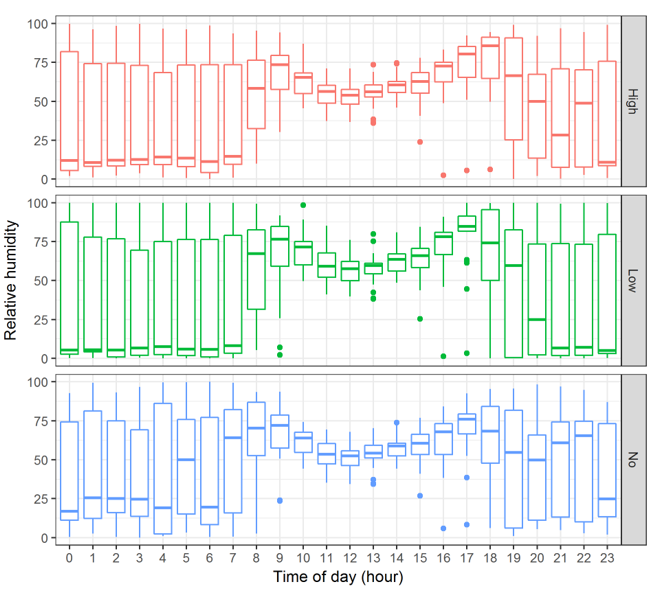
\includegraphics[width=1\textwidth]{Figs/TinyTag}
\caption{\label{fig:tinytags} Data from three `TinyTag' data loggers (Gemini Data Loggers Ltd, Chichester, UK) at canopy height in three of the central treatment arias of the two factor trial during the 21 days preceding panicle harvest.
Showing the treatments high (3 m) in blue, low (ground level) in green and no misting in red.}
\end{figure}


The results from three years of the two factor trial Table \ref{tab:twofactor} shows, in the second year (with misting) the mist applied did have higher seed sets: Ground mist 11\% higher than the control and 3 m mist 18\% higher (p < 0.05) (Table \ref{tab:twofactor}).
In the third year misting did not significantly affect the seed set per m$^2$ (P = 0.45) when tested with a two-way ANOVA.

There was no positive effect from the misting on the germination in the third year (germination was not tested in the second year).
The day of anthesis did not have any detectable effect in the second year and had no significant effect in the third year, analysed with a Friedman rank sum, in the 2$^{nd}$ or 3$^{rd}$ years (P = 1 \& P = 0.76 respectively).
There was naturally no significant effect on plant height or number of panicles in the second or third year (Table \ref{tab:twofactor}).
Also misting has no significant effect on the seed size or weight in the 3$^{rd}$ year (Table \ref{tab:twofactorseed}).


\FloatBarrier
\subsection{Delaying flowering to improve synchronisation}

\FloatBarrier
\subsubsection{Cutting sinensis to synchronise flowering}
To change the flowering time and increase synchronisation, cutting was tested on the \textit{M. sinensis}.

This treatment did significantly (P <0.001) delay anthesis; however, the cutting did lead to a significant (log transformed data, P < 0.001) reduction in panicle numbers, dropping from an average of 60 to 10 panicles per m$^2$ (Table \ref{tab:density}).
This drop in panicle numbers caused by the treatment also explains a drop in seed per m$^2$, which was significantly affected when tested with a two-way ANOVA for density and cut (P < 0.01 \& P < 0.05).
Seed per panicle was significantly (P < 0.001) higher in cut plants, on average 3 times higher, this was primarily prominent in the highest density plants having lots more seed per panicle when cut (Table \ref{tab:density}).
This also manifested in a significant interaction with density (P < 0.001).
However this positive effect maybe due to the cut plants not lodging and thus being more able to accept pollen form the \textit{M. sacchariflorus}.

Testing the germination of the 2018 seed revealed a large significant (P < 0.01) drop in germination (56\% to 34\%) on the parts of the density trial with cutting, likely be due to the plants being weaker and lass able to make viable seed.
This germination issue makes cutting a worse prospect for flowering synchronisation when done to the seed parent.

The MARVIN produced seed metrics showed significant effects on the seed of the cutting treatment (Table \ref{tab:densityseed}).
The seed from cut plants was smaller (P < 0.01) both in length (P < 0.05) and width (P < 0.01) and weighed less (P < 0.05).
These notable seed size differences are likely what lead to the poor germination as the plant complete seed maturation.



\FloatBarrier
\subsubsection{Cutting sacchariflorus}
The cutting of the \textit{M. sacchariflorus} was done primarily to increase panicle numbers and align the heights of the typically smaller \textit{M. sinensis} and taller \textit{M. sacchariflorus}.
Cutting was tested in the first year on the two factor trial (Figure \ref{fig:twoFactorPlan}), with three heights and two times.

The cutting of the \textit{M. sacchariflorus} at differing heights had no significant effect and twice vs once had no significant effect on  the plant height at the end of the season.
However, by end of the season overall cutting (either once or twice) vs not cutting resulted in a large significant (P < 0.001) difference in height of plants 1 - 1.3 m to an average height of 3.4 m from 2.4 m  (Table \ref{tab:sacccut}).
There was unexpectedly no effect on the number of panicles (P = 0.22) (Table \ref{tab:sacccut}).
This lack of extra panicles is odd as \textit{M. sacchariflorus} produces side shoots from stem nodes if cut.
This lack of panicles may be because side shoots produced did not have time to mature and flower before the day-length for flowering initiation was reached.

There was also a significant effect when the day of anthesis was analysed with a two-way ANOVA the cutting two times significantly (P < 0.01) delayed the day of anthesis (~10 days).
However, the height of the cutting did not have a significant effect (P = 0.07).
This was likely due to the strong dependency on day length for flowering in \textit{M. sacchariflorus} \citep{Jensen2013,Deuter2000}.
The distinct advantage to cutting the \textit{M. sacchariflorus} was the more closely harmonised heights when compared to the \textit{M. sinensis}, this may allow better pollen transfer between the species.


\begin{table}[ht]\tiny
\renewcommand{\arraystretch}{1.3}
\caption{This gives the results of the cutting of the \textit{M. sacchariflorus} in two factor trial in 2016.
$n = 2$}
\centering
\begin{tabular}{S   S    S   S  }
\toprule
\multicolumn{2}{c }{\textbf{Cutting \textit{M. sacchariflorus}}} & \multicolumn{1}{c }{\textbf{Plant height (m)}}& \multicolumn{1}{c }{\textbf{Panicles (per m$^2$)}} \\
\textbf{Cut height (m)} & \textbf{Number of times}  & \textbf{Mean} $\pm$ \textbf{SE} & \textbf{Mean} $\pm$ \textbf{SE}\\
\midrule
\multicolumn{2}{c }{Control} & 	3.4$\pm$0.12		& 5$\pm$0.4 \\
1	& 1		& 	3.6$\pm$0.14		& 4$\pm$0.9 \\
2	& 2		& 	2.2$\pm$0.09		& 5$\pm$0.6 \\
0.5	& 1   	& 	2.4$\pm$0.02		& 6$\pm$0.5 \\
0.5	& 2		& 	1.9$\pm$0.02		& 6$\pm$0.5 \\
0.3	& 1		& 	2.1$\pm$0.11		& 5$\pm$1.0 \\
\toprule
\end{tabular}
\label{tab:sacccut}
\end{table}
 

Cutting back the \textit{M. sacchariflorus} was also tested using crenulations in the ratio trial.
In this trial there was no significant effect of this cutting on panicle numbers when tested with a Kruskal-Wallis rank sum in the ratio trial (P = 0.89).
The flowering time measured as the first day anthesis was recorded was not significantly affected by this cutting, averaging to the 25$^{th}$ of October for cut and uncut \textit{M. sacchariflorus} alike (SE 0.9 and 2.3 days respectively).
In this case as cutting was only to a height of 1 m and was done just once, a prominent effect on flowering time was therefore unlikely.



\FloatBarrier
\subsubsection{Nitrogen application to synchronise flowering}
\title{Field testing of Nitrogen}

In the third and fourth years there was not a significant (P = 0.44) effect from nitrogen on the flowering time as measured by the day of anthesis when tested with a Friedman rank sum (Table 6).
This result could be due to the prill used to apply the nitrogen to the plants, as in the dry climate of Catania the prill being dissolved was reliant primarily on the irrigation system.
This may have made the results of the nitrogen more inconsistent.

Nitrogen had a small significant (P < 0.05) effect on the height of the plants in the third year.
The height was only reduced at the highest nitrogen level, equivalent to 130 kg ha$^{-1}$.
In the fourth year the plant heights were not recorded due to the impenetrability of the plot after 4 years of growth.
The effect of nitrogen may be due to increased weed competition when there is a lot of nitrogen in the soil around the plant.


\begin{table}[ht]\tiny
\renewcommand{\arraystretch}{1.3}
\caption{The results from three years of the two factor trial.
Per m$^2$ gives the average amount per m$^2$ of whithin each harvest area. $n = 2$} % n = 3?
\centering
\begin{tabular}{l l  S[table-format=3] S  S[table-format=2]  S}
\toprule
\multicolumn{2}{c }{Year} & \multicolumn{1}{c }{\textbf{Anthesis (DoY)}} & \multicolumn{1}{c }{\textbf{Plant Height (m)}}& \multicolumn{1}{c }{\textbf{panicles (per m$^2$)}}& \multicolumn{1}{c }{\textbf{Seed (g m$^{2 -1}$)}} \\
\textbf{Main treatment} & \textbf{Sub treatment} & \textbf{Mean} $\pm$ \textbf{SE}  & \textbf{Mean} $\pm$ \textbf{SE} & \textbf{Mean} $\pm$ \textbf{SE} & \textbf{Mean} $\pm$ \textbf{SE}\\
\midrule
\multicolumn{2}{c }{\textbf{2$^{nd}$year}} \\
\textbf{Misting}\\ 
\hdashline[2.5pt/3pt]
Control		&           &273 $\pm$0		&2.22 $\pm$0.06 	&26 $\pm$2.5 	&1.08   $\pm$0.12 		\\
Ground mist	&           &273 $\pm$0		&2.31 $\pm$0.04 	&27 $\pm$2.9 	&1.2    $\pm$0.2		\\
3m mist		&           &273 $\pm$0		&2.30 $\pm$0.05 	&29 $\pm$2.6 	&1.32 	$\pm$0.08	    \\
\midrule
\multicolumn{2}{c }{\textbf{3$^{rd}$ year}} \\
\textbf{Misting} & \textbf{Nitrogen}\\ 
\hdashline[2.5pt/3pt]
Control		& Control 	&283 $\pm$0.4	&2.14 $\pm$0.05		&44 $\pm$5.5	&0.69 $\pm$0.20 \\
Control		& Low 		&283 $\pm$0		&2.22 $\pm$0.02		&25 $\pm$2.4	&0.66 $\pm$0.07 \\
Control		& High 		&283 $\pm$0.4	&2.15 $\pm$0.02		&32 $\pm$3.0	&0.45 $\pm$0.03 \\
Ground mist	& Control 	&283 $\pm$0.4	&2.24 $\pm$0.03		&27 $\pm$2.1	&0.47 $\pm$0.04 \\
Ground mist	& Low 		&282 $\pm$0.9   &2.23 $\pm$0.02		&29 $\pm$3.4	&0.37 $\pm$0.02 \\
Ground mist	& High 		&286 $\pm$1.7	&2.13 $\pm$0.03		&39 $\pm$6.5	&0.75 $\pm$0.26 \\
3m mist		& Control 	&283 $\pm$0 	&2.23 $\pm$0.02		&26 $\pm$0.4	&0.51 $\pm$0.06 \\
3m mist		& Low 		&284 $\pm$0.9	&2.25 $\pm$0.06		&40 $\pm$1.9 	&0.63 $\pm$0.15 \\
3m mist		& High 		&283 $\pm$0		&2.10 $\pm$0.11		&22 $\pm$3.3	&0.50 $\pm$0.05 \\
\midrule
\multicolumn{2}{c }{\textbf{4$^{th}$ year}} \\
\textbf{Drought} & \textbf{Nitrogen}\\ 
\hdashline[2.5pt/3pt]
Control		& Control 	&273 $\pm$1.7$^a$   & 			        &46 $\pm$5.3    &0.72 $\pm$0.25 \\
Control		& Low 		&273 $\pm$1.8$^a$   & 			        &22 $\pm$5.1    &0.33 $\pm$0.16 \\
Control		& High 		&272 $\pm$3.5$^a$   & 			        &41 $\pm$16.7   &0.79 $\pm$0.42 \\
50\%		& Control 	&275 $\pm$0.4$^{ab}$   & 			        &33 $\pm$4.4	&0.41 $\pm$0.09 \\
50\%		& Low 		&275 $\pm$0$^b$	    & 			        &24 $\pm$4.5	&0.31 $\pm$0.05 \\
50\%		& High 		&275 $\pm$0$^b$     & 			        &32 $\pm$2.7	&0.61 $\pm$0.04 \\
25\%		& Control 	&275 $\pm$0$^b$     & 			        &21 $\pm$1.6	&0.27 $\pm$0.04 \\
25\%		& Low 		&274 $\pm$0.6$^c$   & 			        &25 $\pm$1.5	&0.35 $\pm$0.05 \\
25\%		& High 		&274 $\pm$0.5$^c$   & 			        &28 $\pm$6.7	&0.47 $\pm$0.16 \\
\toprule
\end{tabular}
\label{tab:twofactor}
\end{table}



\begin{table}[ht]\tiny
\renewcommand{\arraystretch}{1.3}
\caption{The seed results two years of the two factor trial. $n = 2$} % n = 3?
\centering
\begin{tabular}{l l  S S  S  S}
\toprule
\multicolumn{2}{c }{Year} & \multicolumn{1}{c }{\textbf{Weight (mg)}} & \multicolumn{1}{c }{\textbf{Length (mm)}}& \multicolumn{1}{c }{\textbf{Width (mm)}}& \multicolumn{1}{c }{\textbf{Area (mm$^2$)}} \\
\textbf{Main treatment} & \textbf{Sub treatment} & \textbf{Mean} $\pm$ \textbf{SE}  & \textbf{Mean} $\pm$ \textbf{SE} & \textbf{Mean} $\pm$ \textbf{SE} & \textbf{Mean} $\pm$ \textbf{SE}\\
\midrule
\multicolumn{2}{c }{\textbf{3$^{rd}$ year}} \\
\textbf{Misting} & \textbf{Nitrogen}\\ 
\hdashline[2.5pt/3pt]
Control		& Control 	&1.05 $\pm$0.03	&0.94 $\pm$0.02		&2.36 $\pm$0.03	&1.93 $\pm$0.03 \\
Control		& Low 		&0.88 $\pm$0.01	&0.89 $\pm$0.01		&2.24 $\pm$0.01	&1.74 $\pm$0.02 \\
Control		& High 		&1.03 $\pm$0.03	&0.98 $\pm$0.02		&2.35 $\pm$0.03	&1.93 $\pm$0.04 \\
Ground mist	& Control 	&1.07 $\pm$0.04	&0.98 $\pm$0.02		&2.35 $\pm$0.02	&1.95 $\pm$0.05 \\
Ground mist	& Low 		&1.08 $\pm$0.03 &0.98 $\pm$0.01		&2.36 $\pm$0.02	&1.98 $\pm$0.03 \\
Ground mist	& High 		&0.96 $\pm$0.03	&0.95 $\pm$0.01		&2.30 $\pm$0.04	&1.88 $\pm$0.05 \\
3m mist		& Control 	&1.14 $\pm$0.01	&0.98 $\pm$0.01		&2.40 $\pm$0.02	&2.01 $\pm$0.02 \\
3m mist		& Low 		&1.10 $\pm$0.03	&0.98 $\pm$0.02		&2.42 $\pm$0.02	&2.04 $\pm$0.02 \\
3m mist		& High 		&1.05 $\pm$0.07	&0.98 $\pm$0.01		&2.39 $\pm$0.01	&2.02 $\pm$0.02 \\
\midrule
\multicolumn{2}{c }{\textbf{4$^{th}$ year}} \\
\textbf{Drought} & \textbf{Nitrogen}\\ 
\hdashline[2.5pt/3pt]
Control		& Control 	&0.99 $\pm$0.05 &2.17 $\pm$0.05     &0.88 $\pm$0.03 &1.65 $\pm$0.03 \\
Control		& Low 		&1.00 $\pm$0.03 &2.20 $\pm$0.00     &0.88 $\pm$0.03 &1.65 $\pm$0.03 \\
Control		& High 		&1.01 $\pm$0.04 &2.18 $\pm$0.03     &0.88 $\pm$0.03 &1.68 $\pm$0.06 \\
50\%		& Control 	&0.91 $\pm$0.06 &2.12 $\pm$0.05     &0.88 $\pm$0.03	&1.55 $\pm$0.06 \\
50\%		& Low 		&1.08 $\pm$0.05	&2.28 $\pm$0.03     &0.90 $\pm$0.00	&1.82 $\pm$0.05 \\
50\%		& High 		&1.03 $\pm$0.03 &2.22 $\pm$0.05     &0.90 $\pm$0.00	&1.72 $\pm$0.03 \\
25\%		& Control 	&1.14 $\pm$0.02 &2.25 $\pm$0.03     &0.93 $\pm$0.03	&1.78 $\pm$0.03 \\
25\%		& Low 		&1.06 $\pm$0.05 &2.25 $\pm$0.03     &0.90 $\pm$0.00	&1.75 $\pm$0.05 \\
25\%		& High 		&0.95 $\pm$0.04 &2.18 $\pm$0.03     &0.85 $\pm$0.03	&1.60 $\pm$0.04 \\
\bottomrule
\end{tabular}
\label{tab:twofactorseed}
\end{table}


There was no significant effect from nitrogen on the germination of the 33$^{rd}$ or 43$^{th}$ year seed; however, there was a significant (p < 0.05) but detrimental effect which was that the chance of un-germinated seeds going mouldy increased with higher nitrogen (a 16 total increase).
This effect was not unforeseen as there may be more available nitrogen in the seed and this will provide more resources to potential mould.
However, this effect was not significant in the fourth year.

In the third year of the two factor trial there was no significant effect of nitrogen on the number of panicles or seed produced per m$^2$ for harvest, this was also true in the fourth year where neither were significantly affected by the nitrogen application (Table 6).
Also in the third year nitrogen did not significantly affect the weight, width, length or area of the seeds (Supplementary Table 1).
The only significant effect on the seed from nitrogen in the fourth year was a significant interaction with the drought treatment on the seed size and weight (P < 0.01 \& P < 0.05 respectively).
This appears to show that plants with low nitrogen and drought produced the bigger seeds; while significant this effect is small (Supplementary Table 1).
This could show the plant providing more resources to the seed when the environment is challenging.




\FloatBarrier
\title{Greenhouse testing of nitrogen}

PCH-14 (\textit{M. sinensis} side) and PCH-3 (\textit{M. sacchariflorus} side) had nitrogen applications at the same level per plant as in Catania (37$^{\circ}$N).
This was done in parallel with the field trial to test the flowering time in a more controlled environment.
It was expected that the increase in nitrogen would delay the flowering and this would be easier to observe in the glasshouse.

The Nitrogen (ammonium nitrate (34.5\% N)) was diluted in 300 ml of water and applied to the base of the stem for each plant.
The amount of nitrogen used was 0, 41.48 and 83.74 g per plant, this was to mirror the amounts used per plant in Catania to achieve equivalents of 0, 65 and 130 kg per ha.
The PCH-14 plants were grown in a light controlled glasshouse simulating the Catania day-length (37$^{\circ}$N), while the PCH-3 plants were grown in a naturally lit glasshouse in Aberystwyth.
All plants received the 300ml of water, then were left for 24h to absorb the water before manual bottom up watering was started by filling all the trays for the female plant when they became empty.
Plants were only watered when they all became empty.
Males were manually watered top down.
Flowering was scored three times a week making the glasshouse data able to detect more subtle changes in flowering time than the weekly field data.

Due to the fertiliser not being acidity regulated (as it was in the Catania trial) there was a large confounding effect of the acidity that made the highest level of nitrogen non applicable for study.
The \textit{M. sacchariflorus} form PCH-3 did not flower so will also be excluded.

The flowering times of the PCH-14 \textit{M. sinensis} plants were not significantly altered by the nitrogen (P = 0.23); the average time until anthesis was approximately the same which was one day different.
The start of flowering (flag leaf) was also not significantly affected by the nitrogen (P = 0.37).
The nitrogen did not significantly affect the number of panicles or the number of non-flowering stems the plant produced.

These results supported the findings of the Nitrogen trial in Catania (37$^{\circ}$N).
While both this and the field experiment had notable shortcomings, neither seeing a significant effect seems to suggest that any change in flowering time in PCH-14 would be so small as to not benefit flowering synchronisation.



\FloatBarrier
\subsubsection{Droughting to synchronise flowering}
The plants showed signs of yellowing in blocks with the higher drought intensities; however, the drought may have been more successful if more severe as the flowering was more delayed than advanced by the drought as predicted.
If droughting was used to improve flowering synchronisation successfully at all it would need to be used on the pollen parent as a drought below 25\% of evapotranspiration would have an effect on the health of the plants which may affect the panicle numbers and seed set.
Any reduction in the health of the plants suffering under the drought was not seen in the fourth year two factor experiment with no significant effect on the germination of ether the \textit{M. sinensis} or \textit{M. sacchariflorus} seed which remained around 41\% when tested in seven day germination tests.
There was also no significant effect on the seed size or weight from drought alone (Table 8), there was an interaction with nitrogen that suggested the plants may produce bigger seed in difficult conditions.

Table 9: The effect on panicle number, seed amounts and seed MARVIN information of droughting the \textit{M. sacchariflorus} in 2018.
Seed width has not been shown as it was always found to be 0.7 mm for all treatments.
Data shown with the means $\pm$ SE with n = 4.
 

In this case the number of \textit{M. sinensis} panicles and amount of seed was not significantly changed by the drought treatments in the 4th year of the two factor trial (Table 6).
The panicles per m$^2$ of \textit{M. sacchariflorus} plants that also experienced the drought, were also not significantly affected producing 4$\pm$1.5, 5$\pm$0.8, 3$\pm$0.7 panicles per m$^2$ at 25\% evapotranspiration, 50\% evapotranspiration and 100\% evapotranspiration respectively (Table 9).
While the seed and panicles per m$^2$ were broadly the same there was a notable decrease at 25\% evapotranspiration replacement water in the amount of seed per panicle.
However none of these were significantly different (P = 0.42, P = 0.59, \& P = 0.07 respectively).
This lack of significance was potentially due to the low seed set in the \textit{M. sacchariflorus} from the poor synchronisation in the two factor trial in 2018.
With more plants sampled and a better cross it is likely that a more severe drought may lower the number of seed per panicle.

The MARVIN data on seed size and weight also did not show any significant effects, again this may be limited by the lack of replicates as this was not as comprehensively studied as the reciprocal of the intended cross (Table 9).
The MARVIN data dose show a tendency as seed in the sinensis parent of the plants grown in harsher conditions to produce bigger seeds.

On average PCH-14 produced 369 mg of seed per m$^2$ in 2017, but as an early leading Miscanthus seed based hybrid with poor flowering synchronisation PCH-14 was used to test seed set and flowering synchronisation improvements that could be used when upscaling Miscanthus seed production.
Ideally the amount of seed produced should be more than 2 g per m$^2$ in order to provide enough seed for plugs.
In 2018 PCH-14 control plants produced 0.26 g per m$^2$, a large improvement on some of the 2018 experimental data [from two factor trial] but still lower than the 2017 average and 10$\times$ less than the target 2g per m$^2$.



%%%%%%%%%%%%%%%%%%%%%%%%%%%%%%%%%%%%%%%%%%%%%%%%%%%%%%%%%%%%%%%%%%%%%%%%%%%%%%%%%%%%%%%%%%%%%%%%%%
\FloatBarrier
\section{Discussion}


\FloatBarrier
\subsection{Maximising seed yield methods}
The cutting of the \textit{M. sacchariflorus} had little effect on the flowering but did provide a good way to increase the number of panicles per m$^2$.
There were fewer seed per panicle but there was an increase in seeds per m$^2$.

The method of using morning misting to improve pollen transmission between plants did not increase the amount of seed produced.
This may have been due to the lack of a real increase in humidity (there was no effect measured by humidity sensors) or the droplets from the misting being too large to simulate a morning mist.

The concept of planting the plants closer together (the density trial) or increasing the ratio of the seed parents to the pollen parents (the ratio trial) did not prove to be a long term method for increasing the amount of seeds per m$^2$.
This was because the \textit{M. sinensis} genotype easily lodged after the first year at higher planting densities.
There was still some increase in amount of seed per m$^2$ in these trials but it was not linear with the extra plant material per m$^2$ and commercially lodged plants would be useless for harvesting.

High densities could be used with caution, to increase seed yields per ha, the \textit{M. sinensis} is not ideally suitable for this as the less woody stems are prone to lodging.
Commercially densities would also need to take into account the harvest machinery requirements, as harvesting without cutting the crop is best for sustainable yields.

The ratio produced approximately the same amount of seed regardless of the number of \textit{M. sinensis} rows per pair of \textit{M. sacchariflorus} rows; however, in the second year there was lodging in the trial due to a high planting density.
This trial establishes the ability to be able to put multiple rows of seed parent between rows of pollen parent, without a drop in pollination due to the distance and barrier of the other plants.
This was only tested on \textit{M. sinensis} so the taller \textit{M. sacchariflorus} may be able to have fewer rows between pollen parents.

This ratio trial design is not practical for commercial upscaling because of the interior of the plantation being largely inaccessible due to the high planting density, but lessons from it are able to provide a method for maximising seed production over land area.

\subsection{Improving flowering synchronisation}

cutting sinensis in any commercial use-case would need to be rectified if the cutting was being done on the seed parent (which in this case it was).
For crosses where the primary genotype/seed of interest is harvested from the \textit{M. sacchariflorus} side delaying the \textit{M. sinensis} by cutting, even if that caused a plunge in the number of panicles should still leave sufficient pollen to fertilise many \textit{M. sacchariflorus} panicles.
Applications of this method should also be designed cognisant of the known weakening of \textit{Miscanthus} when repeatedly cut in the summer (green-cuts), the number of panicles may continue to fall year on year as the plants are cut.

Out of the several methods tested to change the flowering synchronisation of the two species the only one with some success was cutting the \textit{M. sinensis}, this gave a ~10 day delay in all flowering stages.
However, this did produce a sharp reduction in the number of panicles, so to be commercially viable the cutting of the \textit{M. sinensis} would need to be improved to provide healthier plants.

The nitrogen and the droughting had no detectable effects on the flowering time of the plants.
There was a small effect from the drought on the \textit{M. sacchariflorus} but this was not the side that needed delaying.
The nitrogen may have failed due to inadequate application, as a per-plant application to a watered plant will always spread out the nitrogen compared to a whole field application.
The droughting may not have been harsh enough to produce the desired effect; particularly as the site had higher than average autumn rainfall.

\subsection{Crossing at different latitudes}
The 28$^{\circ}$N latitude had some effect on the flowering with PCH-3 synchronising better than it did in the first year at 37$^{\circ}$N but the first year of PCH-5 remains approximately the same.
The second site provides commercial security to the process of producing large quantities of Miscanthus seeds.
The is not yet enough evidence to speculate on the effect of the environments on the quantity of seed set per m$^2$ as so much variation is due to the flowering synchronisation.



\section{Recommendations}
\begin{itemize}
    \item Not to plant more than 2-3 rows of seed parent per row of pollen parent until further study of pollen distance.
    \item Not to plant \textit{M. sinensis} at more than 1 plant per m$^2$ to save lodging.
    \item For small <2 week adjustments in flowering time of the pollen parent to use a harsh cut (30-50 cm) 20-25 days prior to flowering (flag leaf).
    \item Cutting could be done in a crenelated manner, and alternated each year to avoid the problems associated with green cutting Miscanthus.
\end{itemize}






%%%%%%%%%%%%%%%%%%%%%%%%%%%%%%%%%%%%%%%%%%%%%%%%%%%%%%%%%%%%%%%%%%%%%%%%%%%%%%%%%%%%%%%%%%%%%%%%%%%%%%
\section{Funding}
The research and development work reported here was supported by ... MUST, Antonella's PhD \& \dots


%%%%%%%%%%%%%%%%%%%%%%%%%%%%%%%%%%%%%%%%%%%%%%%%%%%%%%%%%%%%%%%%%%%%%%%%%%%%%%%%%%%%%%%%%%%%%%%%%%%%%%
\section{Acknowledgments}
The authors also acknowledge the contribution of Terravesta! \& \dots etc \dots

Should Michal Mos be an author?

\section{Data Availability}
All data, is available at \dots OSF.

%%%%%%%%%%%%%%%%%%%%%%%%%%%%%%%%%%%%%%%%%%%%%%%%%%%%%%%%%%%%%%%%%%%%%%%%%%%%%%%%%%%%%%%%%%%%%%%%%%%%%%
\bibliography{references}





\end{document}